%%
% Please see https://bitbucket.org/rivanvx/beamer/wiki/Home for obtaining beamer.
%%
\documentclass[handout]{beamer}
%\usetheme{Warsaw}

\usepackage{blkarray}
\usepackage{bigstrut}
\usepackage{amsmath}
\usepackage{bbm}
\usepackage{harpoon}
\usepackage{caption}
\usepackage{subcaption}
\usepackage[square,numbers]{natbib}
\usepackage{soul}
\setcitestyle{numbers}
\usefonttheme[onlymath]{serif}

\makeatletter
\let\BA@quicktrue\BA@quickfalse
\makeatother

\renewcommand{\vec}[1]{ {\bf #1} }
\newcommand{\mat}[1]{ \vec{#1} }
\newcommand{\abs}[1]{ \left\lvert #1 \right\rvert }

\title{A Supervised Learning Approach to Predicting Multigrid Convergence}
\author[N. Nytko]{Nicolas Nytko\\[3mm]Matthew West, Luke Olson, Scott MacLachlan}
\date{\today}

\begin{document}
\frame{\titlepage}


% Overview
\begin{frame}
  \frametitle{Introduction}
  \begin{itemize}
  \item AMG methods are among fastest today for solving sparse linear systems
  \item Optimal setup for AMG can be difficult, and incorrect parameters could prevent convergence.
    \begin{itemize}
      \item Put careful thought into the problem and selecting relaxation weights, AMG parameters
      \item \st{Just try different values and see what works}
    \end{itemize}
  \item For a specific AMG setup, can we predict efficacy ahead of time?
  \item Look at predicting rate of convergence for specific Poisson, Convection-Diffusion problems.
  \end{itemize}
\end{frame}


% Poisson intro
\begin{frame}
  \frametitle{Poisson Problem}
  \begin{itemize}
  \item Look at the 1D variable coefficients case w/ homogeneous Dirichlet conditions
    \[ -\nabla \cdot \left(k\left(\vec{x}\right) \nabla \vec{y} \right) = f \]
    \[ \Omega = \left[-1, 1\right] \quad \partial\Omega = 0 \]
  \item Discretized on $N=31$ internal points using finite differences, $k\left(\vec{x}\right)$ is discretized on midpoints to preserve symmetry.
  \item For arbitrary C/F splitting, can we predict convergence rate and optimal relaxation weight?
  \end{itemize}
\end{frame}


\begin{frame}
  \frametitle{Training Dataset}
  \begin{itemize}
  \item For ``traditional'' machine learning we need a dataset.
    \pause
  \item Idea: Run a \textit{whole lot} of multigrid iterations.
    \pause
  \item Run multigrid iterations and record convergence rate and relaxation weight for randomly generated C/F splittings and problem setups.
  \end{itemize}
  \begin{center}
    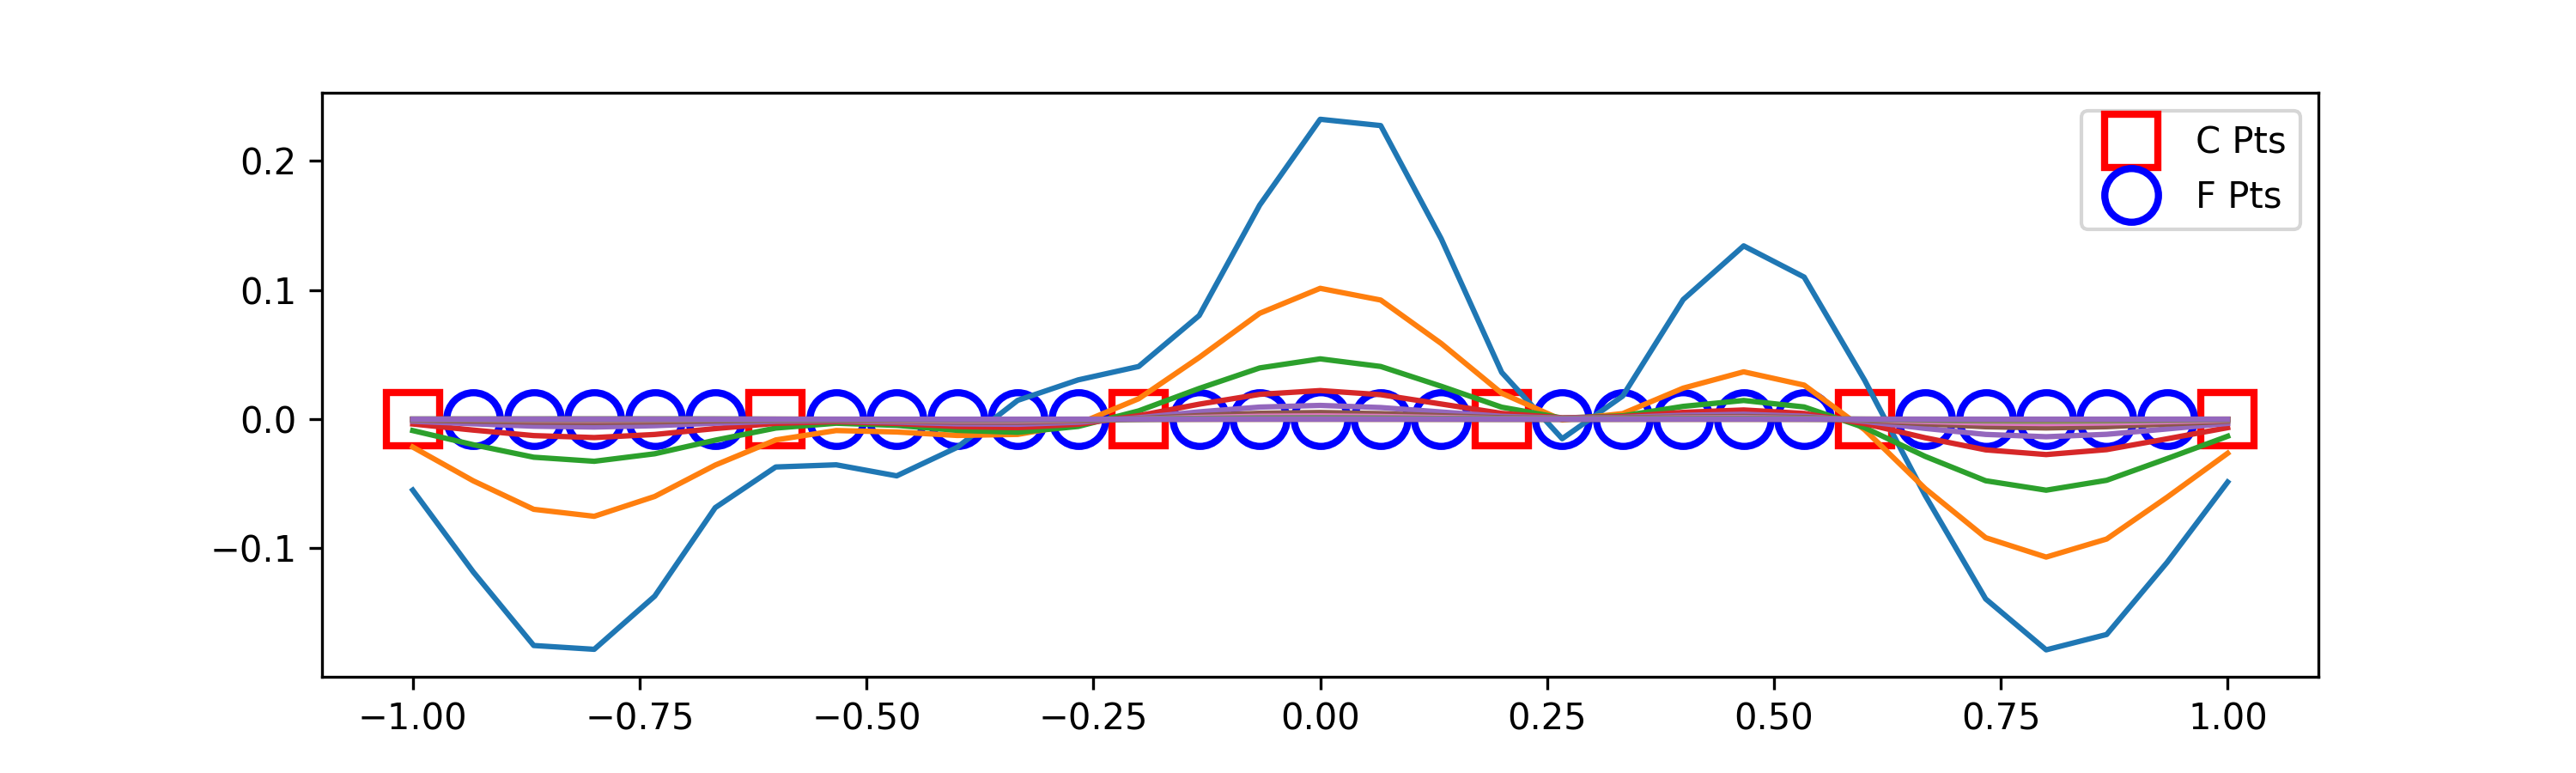
\includegraphics[width=0.8\textwidth]{figures/multigrid.png}
  \end{center}
\end{frame}


\begin{frame}
  \frametitle{Dataset Generation}
  \begin{itemize}
  \item Start from ``reference'' splittings, which are evenly spaced coarse points on a grid.
  \item Randomly perturb each reference in several trials, each point has a set probability of being flipped to opposite value (i.e., coarse to fine and fine to coarse).
  \item Generate variable coefficients according to a few random functions, i.e. cosine wave, random polynomial, noise.
  \end{itemize}
  \begin{figure}[h]
  \centering
  \begin{subfigure}{.48\textwidth}
    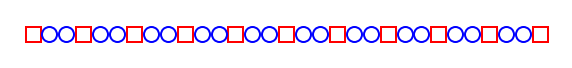
\includegraphics[width=\textwidth]{figures/grid1.png}
    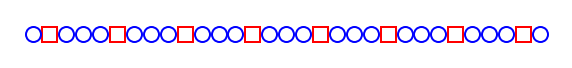
\includegraphics[width=\textwidth]{figures/grid2.png}
    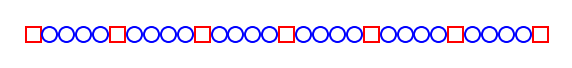
\includegraphics[width=\textwidth]{figures/grid3.png}
    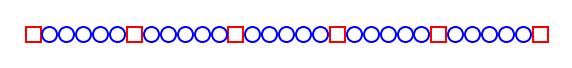
\includegraphics[width=\textwidth]{figures/grid4.png}
    \caption{Various reference grid splittings}
  \end{subfigure}
  \begin{subfigure}{.48\textwidth}
    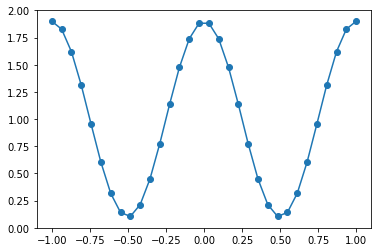
\includegraphics[width=\textwidth]{figures/coeff_ex.png}
    \caption{Example coefficient function}
  \end{subfigure}
  \end{figure}
\end{frame}


\begin{frame}
  \frametitle{Multigrid, CNN}
  \begin{itemize}
  \item Take the C/F splittings, run in multigrid solver to find convergence rate and relaxation weight that maximizes the former.
    \begin{itemize}
    \item Two level V-cycle solver, run for 50 iterations or until error sufficiently small.
    \item Two rounds Jacobi pre- and post-relaxation
    \item Ideal 1D AMG interpolation operator: $\mat{P} = \begin{bmatrix} -\mat{A}_{F\!F}^{-1}\mat{A}_{FC} \\ \mat{I} \end{bmatrix}$
    \end{itemize}
  \item Use the data to train a \textit{1D convolutional network} that predicts convergence, Jacobi relaxation.
    \begin{itemize}
    \item Look at neighboring values of nodes to predict features
    \item Stack multiple CNN layers followed by fully-connected layer to force scalar output
    \end{itemize}
  \end{itemize}
\end{frame}


\begin{frame}
  \frametitle{CNN Performance}
  \begin{figure}[h]
  \centering
  \begin{subfigure}{.48\textwidth}
    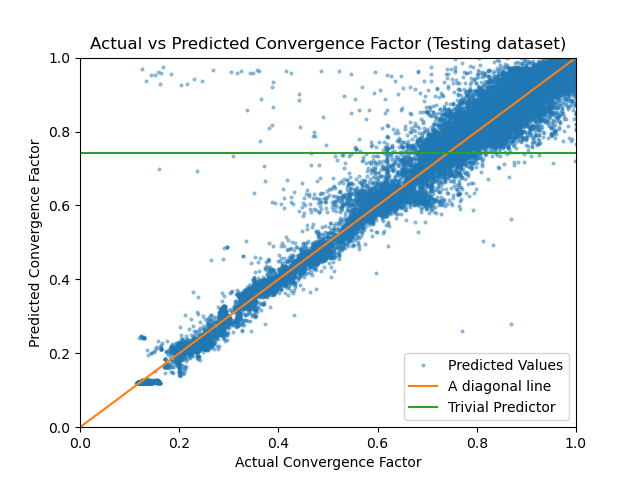
\includegraphics[width=\textwidth]{figures/poisson_conv_test_pred.png}
    \caption{Convergence Factor Predictions}
  \end{subfigure}
  \begin{subfigure}{.48\textwidth}
    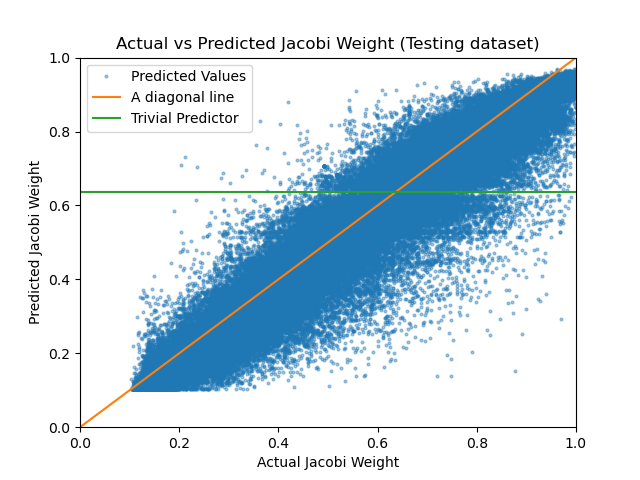
\includegraphics[width=\textwidth]{figures/poisson_jacobi_test_pred.png}
    \caption{Relaxation Weight Predictions}
  \end{subfigure}
  \caption{(a) Predicted convergence values vs. true convergence values, (b) Predicted relaxation weights vs true relaxation weights.  Values closer to the diagonal represent more accurate predictions. }
  \label{fig:poisson_conv_pred}
\end{figure}
\end{frame}


\begin{frame}
  What we learned: \pause Poisson is too easy!
  \newline\newline
  \pause

  Let's try learning a more difficult problem.
\end{frame}


\begin{frame}
  \frametitle{Convection-Diffusion Problem}
  Try out a specific convection-diffusion problem,
  \[\vec{w}\cdot\nabla u -k\nabla^2u = f,\]
  on 2D square, $\Omega = \left[-1,1\right]^2$, discretized as quadrilateral finite elements.  Use  $k=0.1$, $\vec{w} = \begin{bmatrix} 2y(1-x^2) & 2x(1-y^2)  \end{bmatrix}$.  Apply Dirichlet conditions as one ``hot'' wall and three ``cold'' walls.
  \begin{figure}[h]
    \begin{subfigure}{.48\textwidth}
      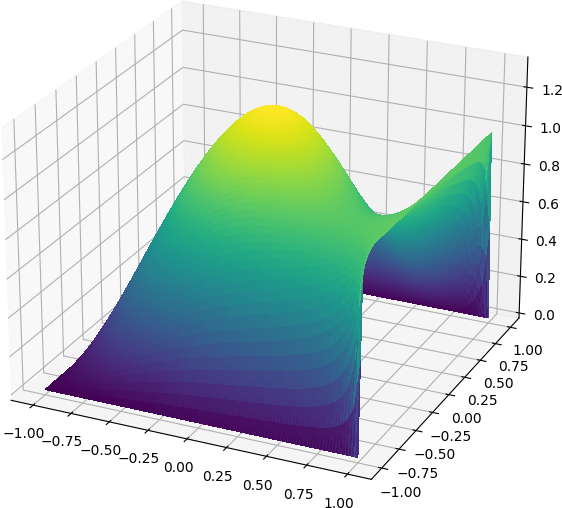
\includegraphics[width=0.9\textwidth]{figures/recirculating.png}
    \end{subfigure}
    \begin{subfigure}{.48\textwidth}
      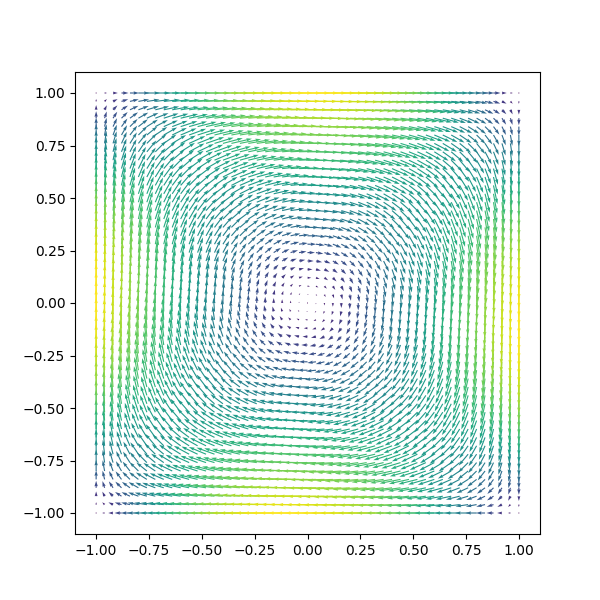
\includegraphics[width=\textwidth]{figures/wind.png}
    \end{subfigure}
  \end{figure}
\end{frame}


\begin{frame}
  \frametitle{Dataset Generation, Convection-Diffusion}
  \begin{itemize}
  \item Discretize on a $25 \times 25$ structured grid.
  \item Start from ``reference'' splittings, all fine, all coarse, AMG output, etc.
  \item Randomly perturb again in various trials.
  \item Don't generate coefficient values for now.
  \item Take output and run through 50 iteration multigrid solver to find convergence rate.
  \end{itemize}
  \begin{figure}[h]
  \begin{subfigure}{.48\textwidth}
    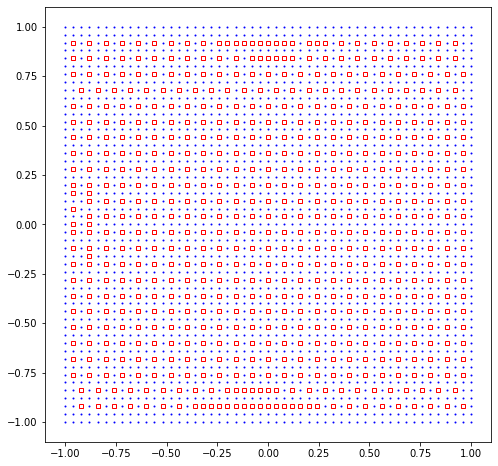
\includegraphics[width=0.8\textwidth]{figures/amgsplit.png}
  \end{subfigure}
  \begin{subfigure}{.48\textwidth}
    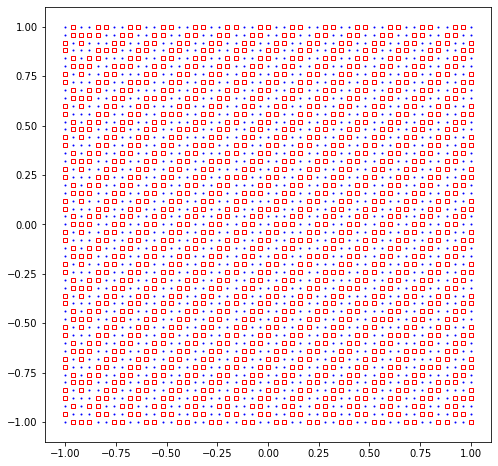
\includegraphics[width=0.8\textwidth]{figures/lin_split.png}
  \end{subfigure}
  \end{figure}
\end{frame}


\begin{frame}
  \frametitle{Convection-Diffusion Convolution}
  \begin{itemize}
    \item 2D structured grid $\Rightarrow$ train 2D convolutional network to predict convergence.
  \end{itemize}
  \begin{figure}[h]
  \centering
  \begin{subfigure}{.48\textwidth}
    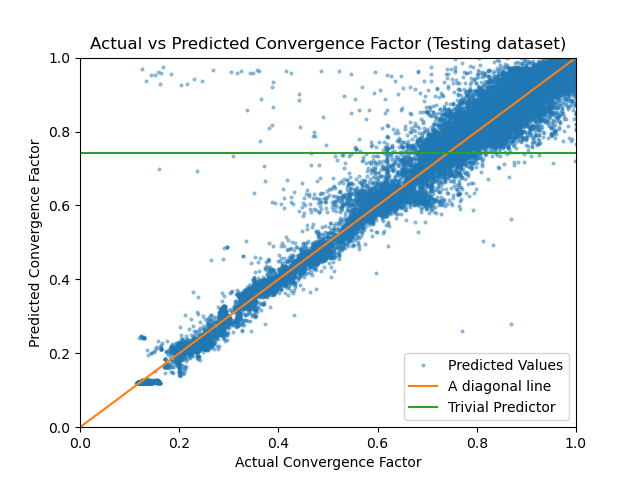
\includegraphics[width=\textwidth]{figures/poisson_conv_test_pred.png}
    \caption{Testing predictions}
    \label{subfig:poisson_conv_test}
  \end{subfigure}
  \begin{subfigure}{.48\textwidth}
    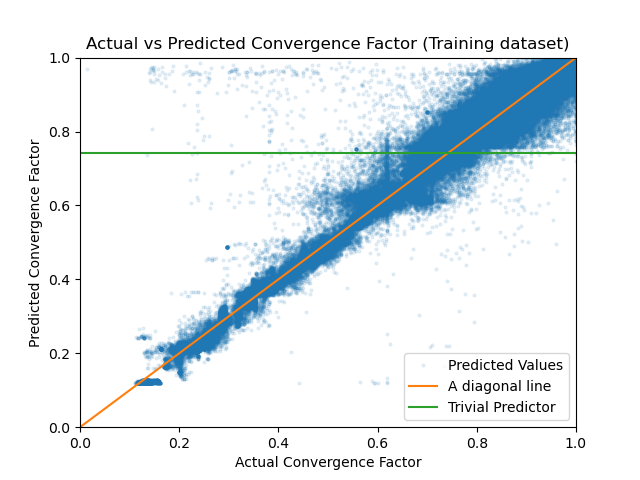
\includegraphics[width=\textwidth]{figures/poisson_conv_train_pred.png}
    \caption{Training predictions}
    \label{subfig:poisson_conv_train}
  \end{subfigure}
  \caption{Predicted convergence values vs. true convergence values on (\ref{subfig:poisson_conv_test}) testing and (\ref{subfig:poisson_conv_train}) training datasets for Poisson equation. Values closer to the diagonal represent more accurate predictions. }
  \label{fig:poisson_conv_pred}
\end{figure}
\end{frame}


\begin{frame}
  \frametitle{CNN to GNN}
  \begin{itemize}
  \item Classical convolution techniques work okay on structured, grid-like inputs.
  \item Very restrictive in terms of mesh data we can use for FEM solvers.
  \item Take a look at some network architectures that allow for unstructured data: introduce \textit{graph-nets}.
    \begin{itemize}
      \item Get FEM matrix, convert to graph and try to learn properties about the system.
    \end{itemize}
  \end{itemize}
    \begin{figure}[h]
  \begin{subfigure}{.4\textwidth}
    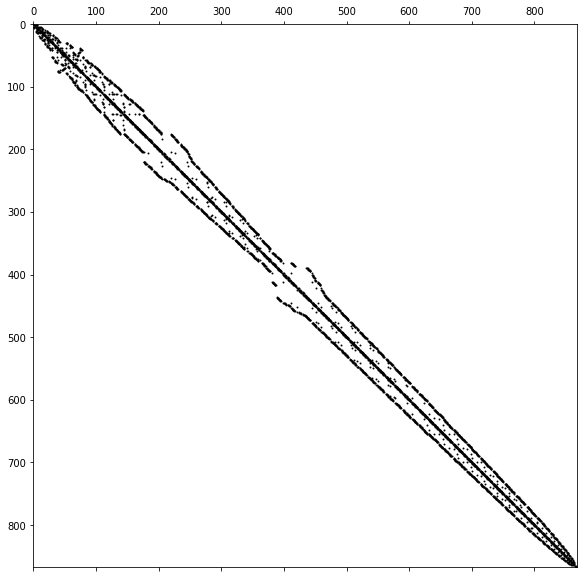
\includegraphics[width=\textwidth]{figures/sparse.png}
  \end{subfigure}
  \begin{subfigure}{.08\textwidth}
    \[ \Longrightarrow \]
  \end{subfigure}
  \begin{subfigure}{.40\textwidth}
    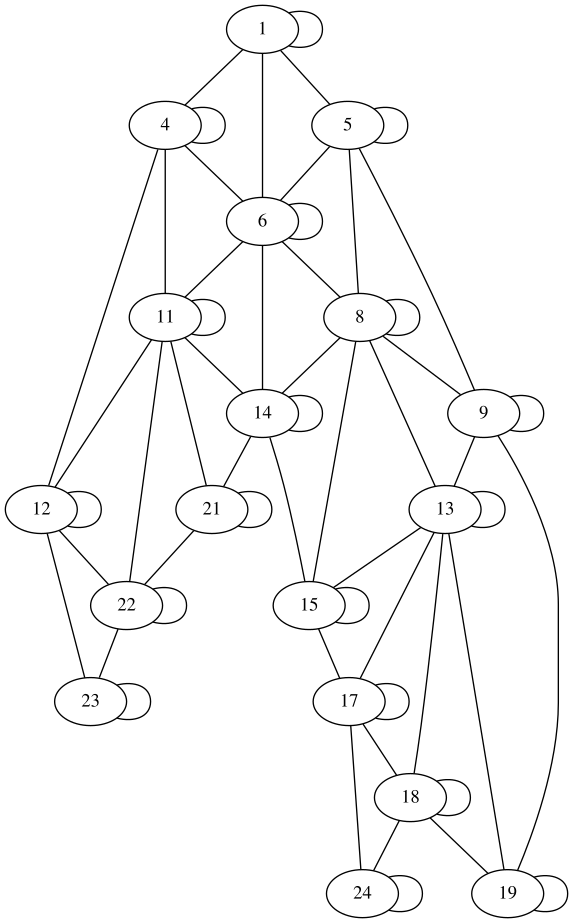
\includegraphics[width=0.6\textwidth]{figures/graph.png}
  \end{subfigure}
\end{figure}
\end{frame}


\begin{frame}
  \frametitle{Message-Passing Graph Convolutions}
  \begin{itemize}
  \item Many graph convolution implementations, one such is the \textit{Message-Passing Graph} layer.
  \item In each layer, nodes learn optimal ``messages'' to pass via edges.  Each node passes this message to other nodes in its neighborhood.
  %% \item Update given by:
  %% \begin{equation*}\label{eqn:mpnn_prop}
  %%   \left(\mat{H}^{(i)}\right)_j = \frac{1}{\abs{\mathcal{N}\left(j\right)}} \sum_{k\in\mathcal{N}\left(j\right)} F^{(i)}\left(e_{j,k}\right)\left(\mat{H}^{(i-1)}\right)_k + \vec{b}^{(i)}
  %% \end{equation*}
  \item Stacking multiple of these layers approximates traditional grid-based convolution.
  \item Run each set of nodal values through linear NN, take average for final convergence rate.
  \end{itemize}
   \begin{figure}[h]
    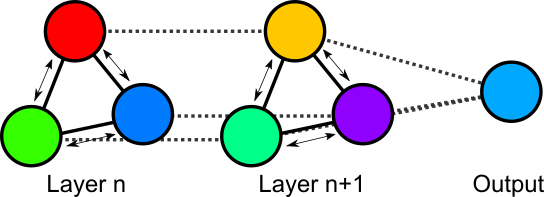
\includegraphics[width=0.5\textwidth]{figures/graphnet.png}
    \caption{Example graphnet architecture}
\end{figure}
\end{frame}


%% \begin{frame}
%%   \frametitle{Message-Passing Architecture}
%%   \begin{itemize}
%%   \item Pass node C/F values, $\mat{X}$, through 4 MPN layers to get $\mat{H}^{(i)}, \enskip i\in\left\{1,2,3,4\right\}$.
%%   \item Stack historical values to both simulate residual-style networks and give more information to aggregator:
%%     \[ \mat{R} =
%% \begin{bmatrix}
%% \hdots & \mat{X}^T & \hdots \\
%% \hdots & \left(\mat{H}^{(1)}\right)^T & \hdots \\
%% \hdots & \left(\mat{H}^{(2)}\right)^T & \hdots \\
%% \hdots & \left(\mat{H}^{(3)}\right)^T & \hdots \\
%% \hdots & \left(\mat{H}^{(4)}\right)^T & \hdots \\
%% \end{bmatrix} \]
%% \item Run each set of nodal values through linear NN, take average for final convergence rate:
%%   \[ y=\frac{1}{N} \sum_j \sigma\left( \left( \vec{r}_j \mat{W}^{(5)} + \vec{b}^{(5)} \right)\mat{W}^{(6)} + \vec{b}^{(6)} \right) \]
%%   \end{itemize}
%% \end{frame}


\begin{frame}
  \frametitle{Message-Passing Dataset}
  \begin{itemize}
  \item Decoupled the neural network from a fixed input size due to final aggregation step.
  \item Can have variable-sized input.  Now generate and train on  a variably-sized dataset of four mesh sizes:
  \[ \left\{ 15\times 15 \quad 25\times 25 \quad 35\times 35 \quad 50 \times 50 \right\} \]
  \end{itemize}
\end{frame}


\begin{frame}
  \frametitle{Message-Passing Performance}
  \begin{figure}[h]
  \centering
  \begin{subfigure}{.48\textwidth}
    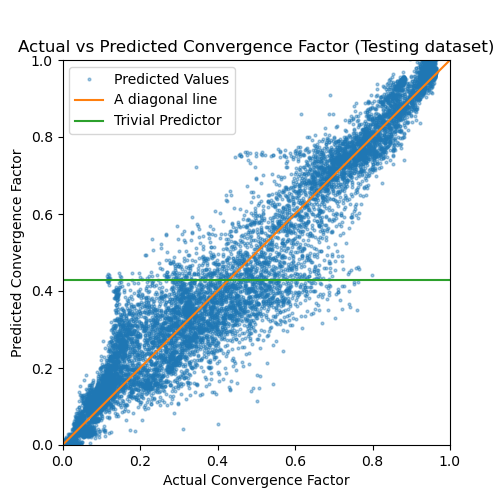
\includegraphics[width=\textwidth]{figures/cd_var_conv_mpnn_test_pred.png}
    \caption{Testing predictions}
    \label{subfig:cd_mpnn_test}
  \end{subfigure}
  \begin{subfigure}{.48\textwidth}
    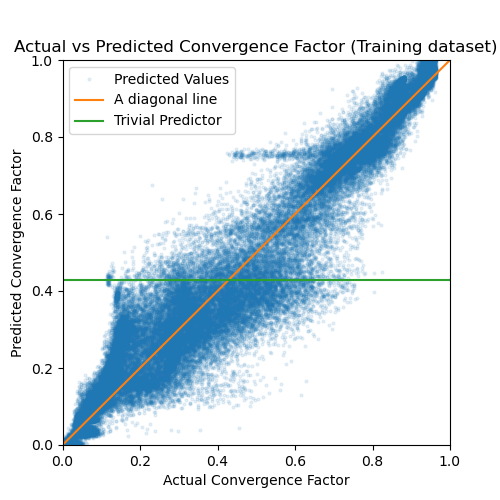
\includegraphics[width=\textwidth]{figures/cd_var_conv_mpnn_train_pred.png}
    \caption{Training predictions}
    \label{subfig:cd_mpnn_train}
  \end{subfigure}
  \caption{Predicted convergence rates vs. true convergence rates on (\ref{subfig:cd_mpnn_test}) testing and (\ref{subfig:cd_mpnn_train}) training datasets for model convection-diffusion problem, using an Edge-Conditioned Convolution network. Values closer to the diagonal represent more accurate predictions.}
  \label{fig:cd_mpnn_pred}
\end{figure}
\end{frame}


%% \begin{frame}
%%   ??? put something here ???

%%   this seems short-ish so far
%% \end{frame}

\begin{frame}
  \frametitle{Conclusions}
  \begin{itemize}
  \item These AMG features are indeed learnable with supervised methods.
  \item Predicting these values becomes more difficult on more complex problems, domains.
  \item What else can we learn?
  \end{itemize}
\end{frame}

\begin{frame}
  \frametitle{Future Directions}
  \begin{itemize}
  \item Try out some more interesting problems:
  \begin{figure}[h]
  \centering
  \begin{subfigure}{.70\textwidth}
    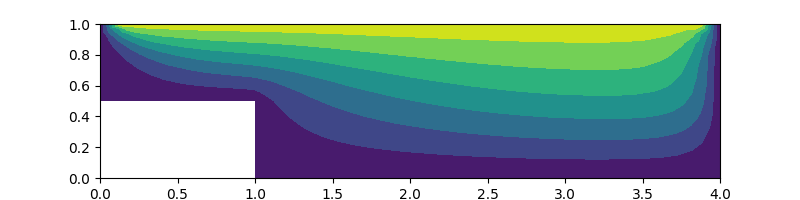
\includegraphics[width=\textwidth]{figures/cd_bfs.png}
  \end{subfigure}
  \begin{subfigure}{.70\textwidth}
    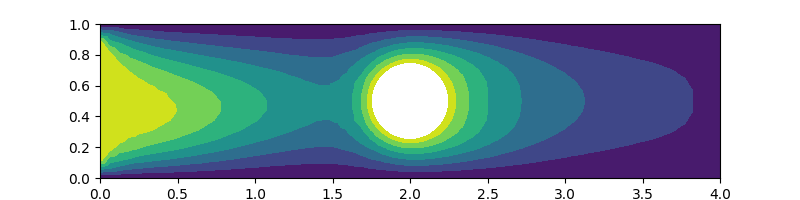
\includegraphics[width=\textwidth]{figures/cd_cyl.png}
  \end{subfigure}
  \end{figure}
  \item Pick between different AMG methods with predictions.
  \item Use predictions in an optimization routine to find most convergent C/F splitting.
  \end{itemize}
\end{frame}

\end{document}
